\section{Electroquasistatic Analysis}
If the induced electric field can be neglected and the displacement currrent \textbf{cannot} (coupling only in one direction $\vec{E} \rightarrow \vec{H}$), the conditions for electroquasistatic analysis are established \\
\begin{equation*}
	\nabla \times \vec{E} = -\frac{\partial \vec{B}}{\partial t} \approx 0
\end{equation*}
\begin{equation*}
	\vec{J} = \underbrace{\vec{J}_s}_{\textrm{source current}} + \underbrace{\sigma \vec{E}}_{\textrm{internal current (conduction)}} + \underbrace{\varepsilon \frac{\partial \vec{E}}{\partial t}}_{\textrm{displacement current (polarization)}}
\end{equation*}
Generally speaking, the
PDE can be obtained with continuity equation $\nabla \cdot \vec{J} = 0$
\begin{equation*}
	\nabla \cdot \left(\sigma \nabla \varphi\right) + \nabla \cdot \left(\varepsilon \frac{\partial}{\partial t}\nabla \varphi\right) = \nabla \cdot \left(\vec{J}_s\right), \textrm{ in } \Omega
\end{equation*}
and PDE in frequency domain
\begin{equation*}
	\nabla \cdot \left(\sigma \nabla \underline{\varphi}\right) + \nabla \cdot \left( j \omega \varepsilon \nabla \underline{\varphi}\right) = \nabla \cdot \left(\vec{J}_s\right), \textrm{ in } \Omega.
\end{equation*}

\textbf{\\ Boundary Value Problem (BVP)\\}
\begin{minipage}[lt]{11cm}
	\begin{tabular}{l}
		\(\displaystyle \varphi = U, \textrm{ over } \partial_{D1}\Omega \) \\
		\(\displaystyle \varphi = 0, \textrm{ over } \partial_{D2}\Omega \) \\
		\(\displaystyle \frac{\partial \varphi}{\partial n} = 0, \textrm{ over } \partial_{N}\Omega \)
	\end{tabular}
\end{minipage}
\begin{minipage}[rt]{8cm}
	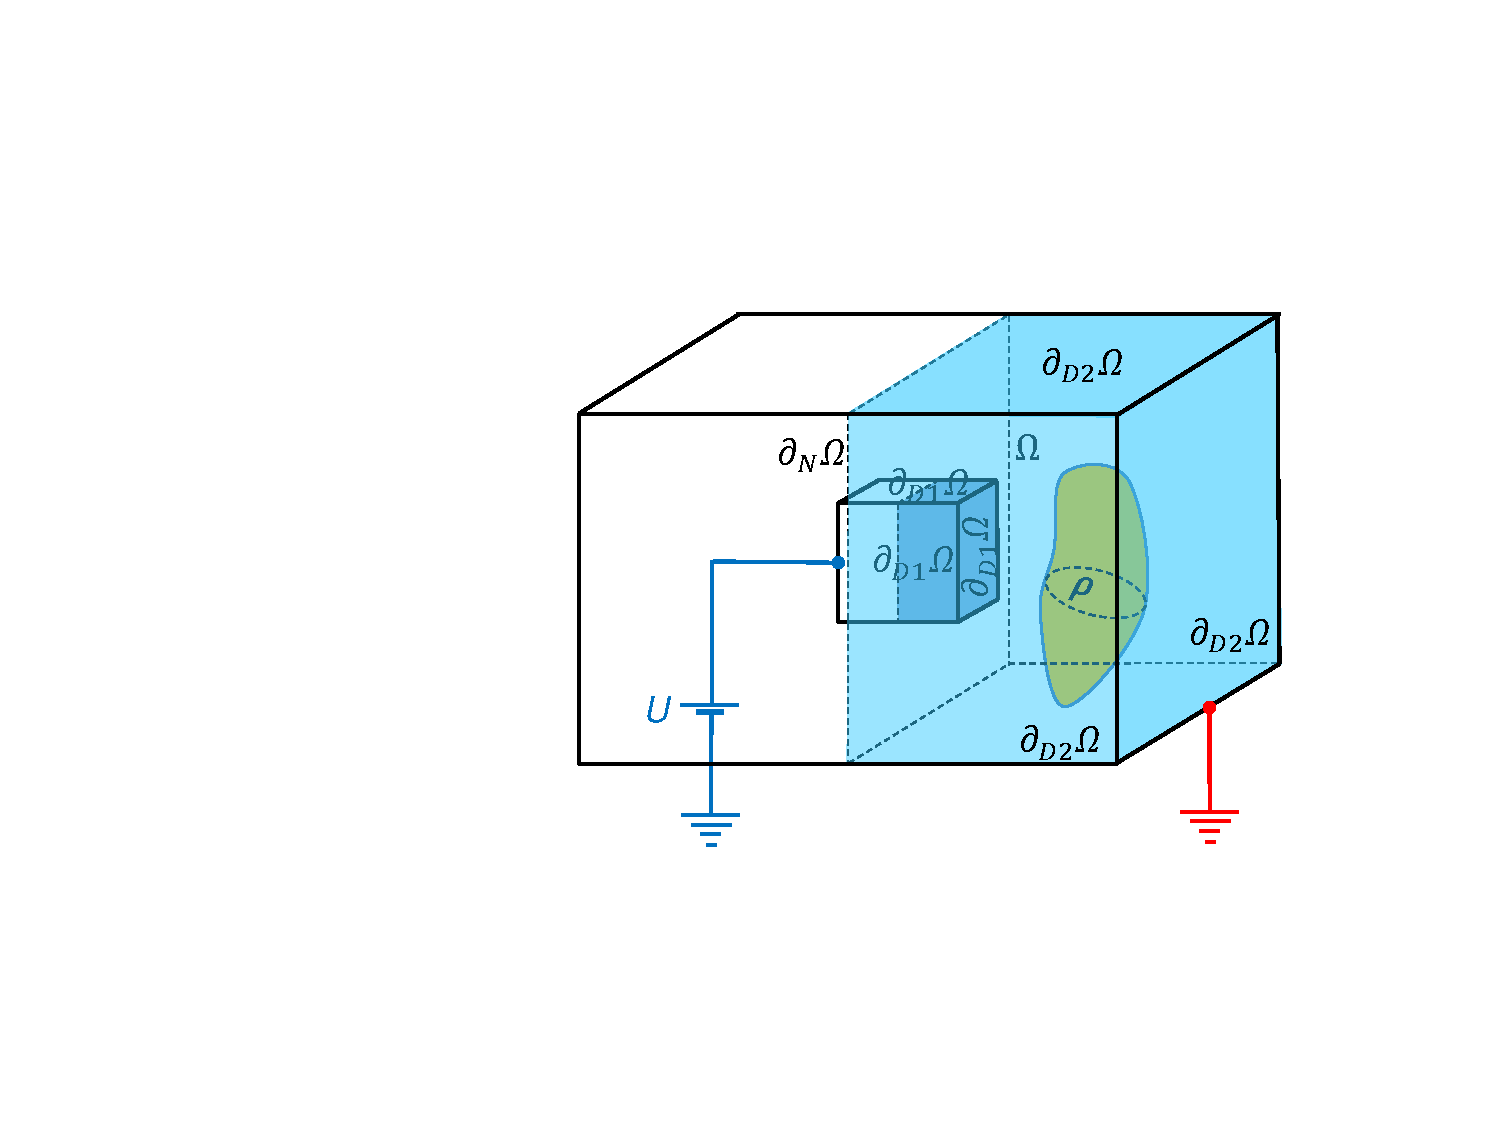
\includegraphics[width=.6\textwidth]{./images/BVP_electrostatic.pdf}
\end{minipage}